\documentclass[conference]{IEEEtran}
\usepackage{graphicx}
\usepackage{amsmath}
\usepackage{caption}
\usepackage{float}

% Title and author
\title{Performance of SPMV Calculation}
\author{Charlie Flux}

\begin{document}
\maketitle

\begin{abstract}
This paper investigates the performance of sparse matrix-vector multiplication (SPMV) using different matrix representations, specifically Coordinate List (COO) and Compressed Sparse Row (CSR), under varying thread counts.
Both parallel and serial implementations are explored, with a focus on the effect of parallelization on execution time.
Results show that CSR outperforms COO in a parallel environment however, COO is more effective in serial applications.
\end{abstract}

\section{Introduction}
The purpose of this experiment is to compare the performance of different matrix representations. Specifically, it examines how varying thread counts affect the performance of parallel sparse matrix-vector multiplication algorithms.
\section{Methodology}
2 Methods of storing matricies were used:
\begin{itemize}
    \item \textbf{Coordinate List (COO)}
    \item \textbf{Compressed Sparse Row (CSR)} 
\end{itemize}

For experiments measuring time, core counts \(C\) were chosen from the set:
    \[
    C = \{1, 2, 4, 6, 8, 12, 16, 24, 32, 48, 64, 96, 128\}
    \]
All experiments used the arguments the matricies provided by cant.mtx \& b.mtx files.
\subsection{Experimental Setup}
All tests were ran on Talepas. Experiments were repeated 20 times and the average was calculated for each experiment. \\
Data was filtered using the Interquartile Range Filter to remove points that do not lie between the first and third quartile as a consequence of the the unreliable data caused by the unlocked variable frequencies on Telepas.

\section{Results}

\subsection{Serial implementation}
Firstly, a serial calculation algorithm was implemented. Figure \ref{fig:serial} shows the performance difference between the CSR and COO formats while calculating the Sparse Matrix-Vector (SPMV) multiplication. As expected, the CSR format performs worse on average due to the $O(n^2)$ time complexity of the algorithm implemented. 
This time complexity is inherent to the CSR method; however, it should become an advantage in a parallel application.
\begin{figure}[H]
    \centering
    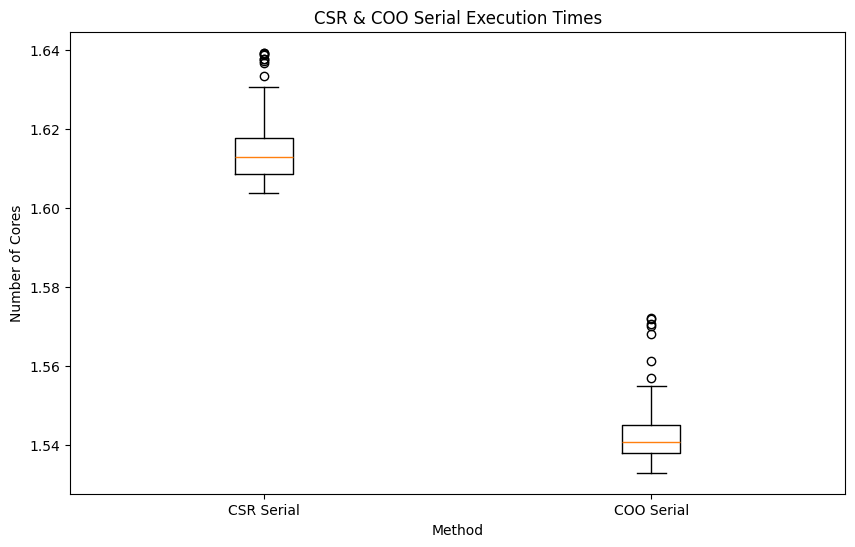
\includegraphics[width=0.45\textwidth]{../img/serial.png}
    \caption{Serial SPMV Implementations}
    \label{fig:serial}
\end{figure}

\subsection{Parallel implementation}
Figure \ref{fig:parallel} has a logarithmic y-axis and compares the execution time of the parallel implementations of the COO \& CSR sparse matrix-vector multiplication algorithms.
In the CSR algorithm, each thread processes an entire row at a time, which improves cache locality and enables more efficient sequential memory access, leading to better performance. In contrast, the COO algorithm uses locks for each row to prevent race conditions when multiple threads access the same row. However, this locking mechanism introduces additional execution overhead. In the CSR algorithm, race conditions are avoided because each row is assigned to an individual thread, eliminating the need for locks.
\begin{figure}[H]
    \centering
    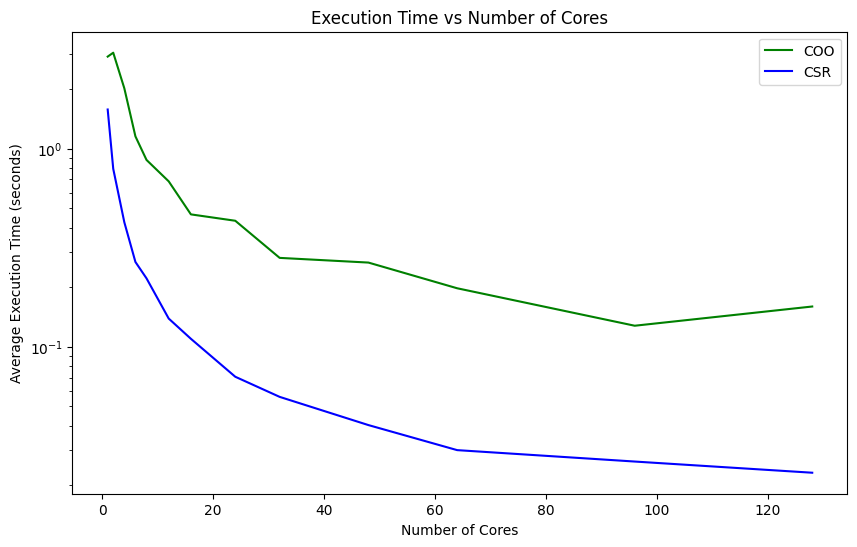
\includegraphics[width=0.45\textwidth]{../img/parallel.png}
    \caption{Parallel SPMV Implementations}
    \label{fig:parallel}
\end{figure}

\subsection{Conversion}
Figure \ref{fig:conversion} illustrates the average execution time for the conversion from COO to CSR formats compared to the number of cores in a parallelized environment. 
A substantial speedup can be found with an increase in core count up to a certain threshold, beyond which the performance gain diminishes, indicating limited scalability of the conversion process at higher core counts.
\begin{figure}[H]
    \centering
    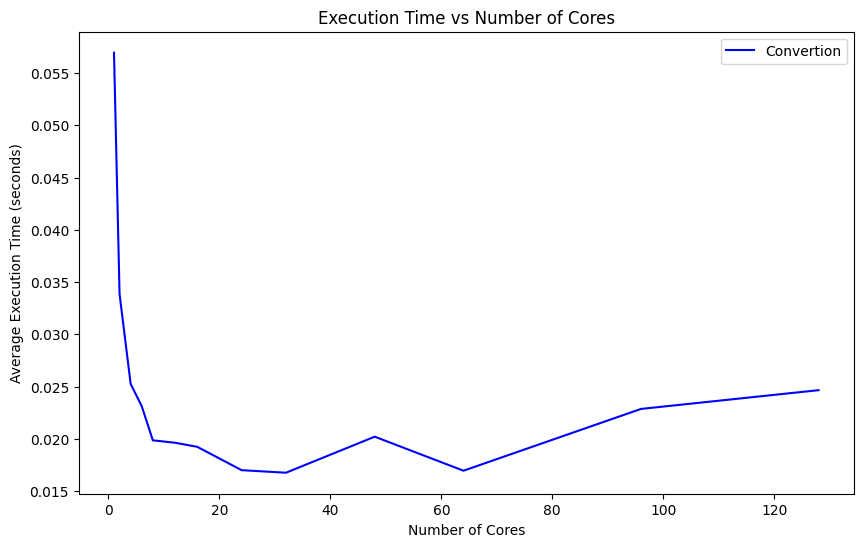
\includegraphics[width=0.45\textwidth]{../img/conversion.png}
    \caption{COO to CSR Conversion}
    \label{fig:conversion}
\end{figure}

\section{Conclusion}

\end{document}
